\chapter{GNBoard design schematics and layout}
\label{Appendix:circuits}
\vspace{-1cm}


\begin{figure}[h!]
\centerline{\mbox{\includegraphics[width=11cm]{images/gnboard_pcb_real.jpg}}}
\captionFigure{Manufactured PCB for the GNBoard v1.0}
{fig:gnboard_pcb_real}{
A total of 20 boards were ordered to \url{http://www.seeedstudio.com/}. The layout utilizes through-hole components solely, in order to simplify the assembly task.
}
\end{figure}




\newpage
%\thispagestyle{empty}
\begin{figure}[h!]
\centerline{\mbox{\includegraphics[width=13.5cm]{images/GNBoard_top.png}}}
\vspace{0.5cm}
\centerline{\mbox{\includegraphics[width=13.5cm]{images/GNBoard_btm.png}}}
\centering\captionFigure{GNBoard v1.0 layout}
{fig:GNBoard_layout}{
Top and bottom views.\\
More information can be found in Section \ref{sect:openSourceElectronics}.
}
\end{figure}





\newpage
\thispagestyle{empty}

\newgeometry{top=3.5cm,bottom=4.5cm,left=1cm,right=0cm}

\begin{landscape}

\begin{figure*}[tb] 
\centering
 \makebox[\textwidth]{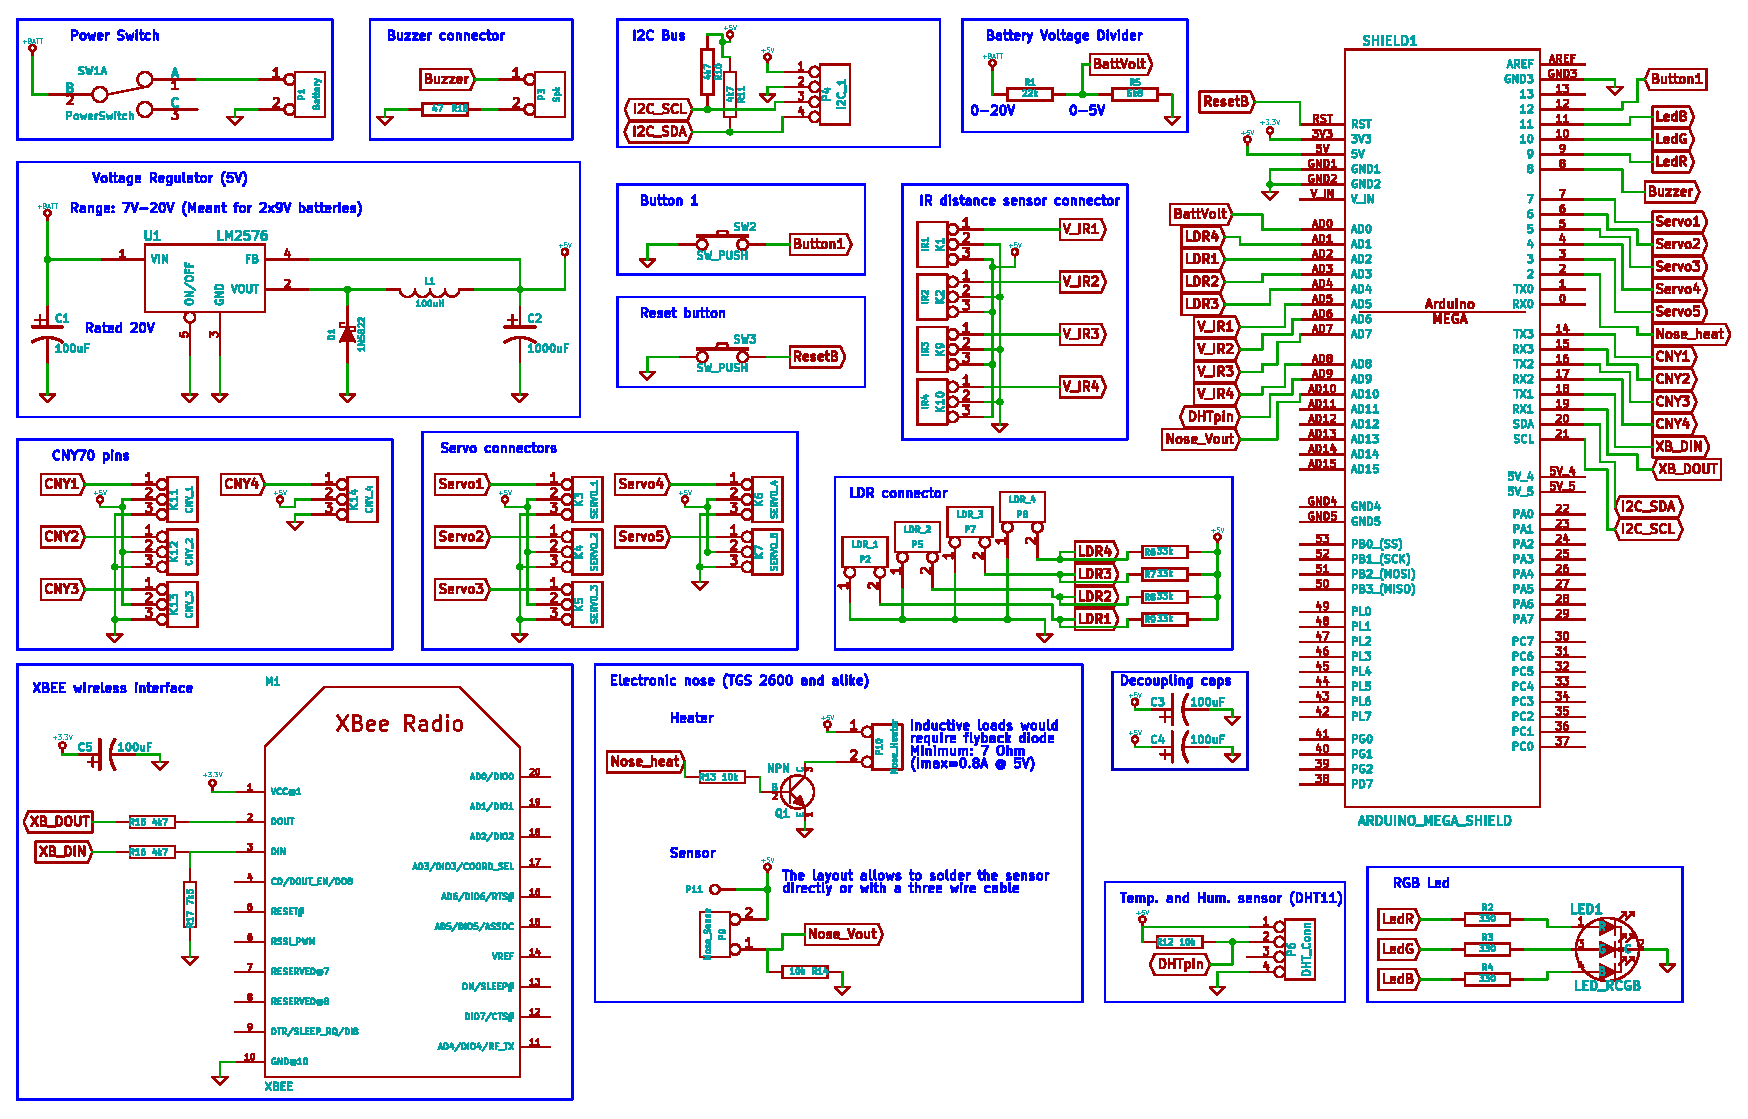
\includegraphics[width=.9\paperheight]{images/GNBoard_schem.eps}}
\captionFigure{GNBoard v1.0 schematic}
{fig:GNBoard_schem}{
More information can be found in Section \ref{sect:openSourceElectronics}.
}
\end{figure*}

\end{landscape}

\restoregeometry

\newpage \thispagestyle{empty} % Página vacía 


